\section{RDDs Essentials}

\subsection{Examples}
\begin{frame}[fragile]
\begin{lstlisting}
	val data = Array(1, 2, 3, 4, 5)
	val distData = sc.parallelize(data)
	
	// add up the elements of the array
	distData.reduce((a, b) => a + b)
	
	// specify number of partitions
	// default: sets automatically based on cluster
	// runs one task for each partition of the cluster
	distData = sc.parallelize(data, 10) 
	
	val distFile = sc.textFile("data.txt")
	
	// add up the sizes of all the lines
	distFile.map(s => s.length).reduce((a, b) => a + b)
	
	// passing functions
	object MyFunctions { def func1(s: String): String = { ... } }
	myRdd.map(MyFunctions.func1)
\end{lstlisting}
\end{frame}

\subsection{Local vs. Cluster}
\begin{frame}[fragile]
\begin{lstlisting}
	var counter = 0
	var rdd = sc.parallelize(data)
	rdd.foreach(x => counter += x)	
	println("Counter value: " + counter)
\end{lstlisting}
\begin{itemize}
  \item Behavior of the above code is undefined
  \item In local mode, works because counter is in the memory of driver
  \item In cluster mode, a new copy of counter is sent to each node in the
  cluster,
  \item In cluster mode, use accumulators to make it work.
  \item Closure: those variables and methods which must be visible for the
  executor to perform its computations on the RDD
  \item The closure is serialized and sent to each executor
\end{itemize}
\end{frame}

\begin{frame}[fragile]
Spark supports ``Shared Variables'' along with RDDs
\begin{itemize}
  \item closure (variable + function) runs in parallel as set of tasks in nodes
  \item generally ships copy of each variable to each task
  \item for sharing across tasks: i) broadcast variables, ii) accumulators
  \item broadcast: cache a value in memory on all nodes
  \item accumulators: variables that are only ``added'', e.g., counters, sums.
\end{itemize}
\begin{lstlisting}
	val broadcastVar = sc.broadcast(Array(1, 2, 3))
	
	val accum = sc.accumulator(0, "My Accumulator")
	sc.parallelize(Array(1, 2, 3, 4)).foreach(x => accum += x)
\end{lstlisting}
\end{frame}

\subsection{RDD Operations}
\begin{frame}
\begin{figure}
\centering
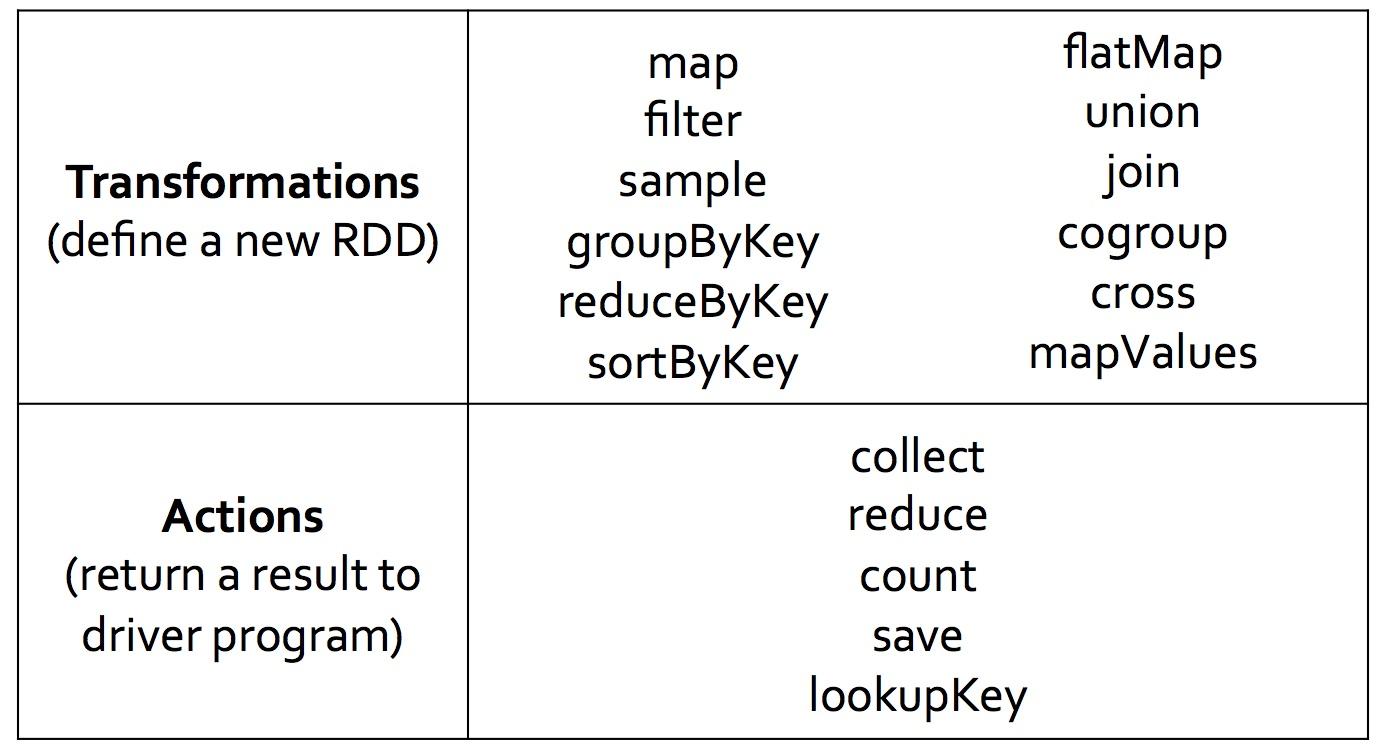
\includegraphics[width=0.80\linewidth]{figures/rdd-operations.jpg}
\caption{Transformations and actions available on RDDs in Spark [2].}
\end{figure}
\end{frame}

\begin{frame}
\begin{figure}
\centering
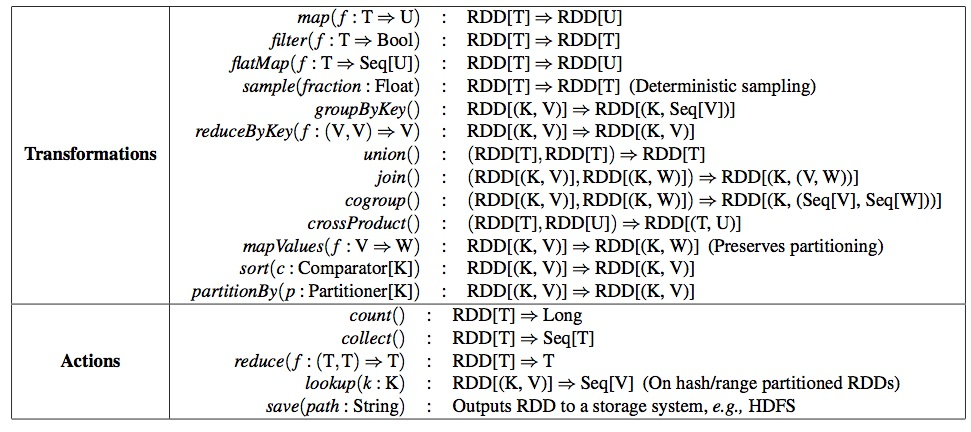
\includegraphics[width=\linewidth]{figures/rdd-operations-details.jpg}
\caption{Transformations and actions available on RDDs in Spark [1].}
\end{figure}
\end{frame}

\subsection{RDD Persistence}
\begin{frame}
\begin{itemize}
  \item Persist RDDs using \texttt{persist()} or \texttt{cache()}
  \item Persisted RDDs can be stored using a storage level
  \item \textit{MEMORY\_ONLY} (default): store RDD as deserialized Java object
  in the JVM, RDD partitions that don't fit will be recomputed
  \item \textit{MEMORY\_AND\_DISK}: similar to before but stores the partitions
  that don't fit on disk
  \item \textit{MEMORY\_ONLY\_SER}: store RDD as serialized Java object
  \item \textit{MEMORY\_AND\_DISK\_SER}: similar but store on disk too
  \item \textit{DISK\_ONLY}: store the RDD partitions only on disk
\end{itemize}
\end{frame}

\begin{frame}
Which storage level to choose?
\begin{itemize}
  \item if RDD fits comfortably with default, leave it as is
  \item if not, try \textit{MEMORY\_ONLY\_SER} and select fast serialization
  library
  \item don't spill to disk unless the functions that computed datasets are
  expensive (otherwise recomputing may be as fast as reading from disk)
  \item use replicated storage level for faster fault recovery
  \item spark automatically monitors cache usage on each node and drops out old
  partitions based on LRU. For manual, \texttt{RDD.unpersist()}
\end{itemize}
\end{frame}

\subsection{RDD Representation}
\begin{frame}
\begin{figure}
\centering
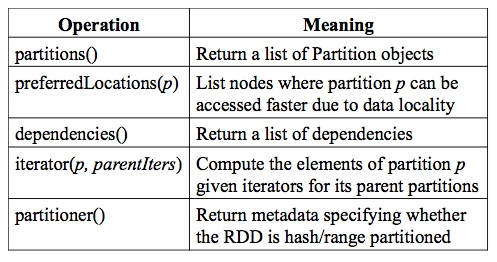
\includegraphics[width=0.55\linewidth]{figures/rdd-representation.jpg}
\end{figure}
RDD interface exposes five pieces of information:
\begin{itemize}
  \item a set of \textit{partitions}, which are atomic pieces of the dataset 
  \item a set of \textit{dependencies} on parent RDDs
  \item a function for computing the dataset based on its parents
  \item metadata about its partitioning
  \item metadata about its data placement
\end{itemize}
\end{frame}

\begin{frame}
Dependencies,
\begin{figure}
\centering
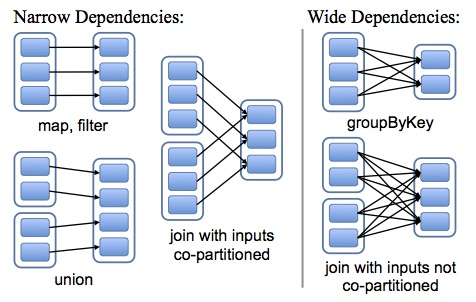
\includegraphics[width=0.45\linewidth]{figures/rdd-dependies.jpg}
\caption{Narrow and wide dependencies [1].}
\end{figure}
%\vpsace{-0.5cm}
Dependencies are useful for,
\begin{itemize}
  \item for staging (seen before, \texttt{groupByKey()})
  \item recovery after node failure, easy with narrow and difficult with wide.
\end{itemize}
\end{frame}

